%=================================================================
%\section{Automated classification of pathology reports into ICD-O codes}

%-----------------------------------------------------------------
%\subsection{Materials and Methods}

\begin{frame}
	\frametitle{Materials and Methods}
	\begin{itemize} \myspacing
		\item 70,000+ documents from 20,000+ patients over 14 years
		\begin{itemize}
			\item Written in Portuguese by Brazilian pathologists
			\item Pathology reports        
                         \item Routine procedure in A.C. Camargo Cancer Center, Brazil
                \end{itemize}
                 \item Gold standard creation
                \begin{itemize}
                		\item Free-text content associated to structured data in cancer registries
			\item Discarded patients with confirmed metastasis or multiple classifications
                \end{itemize}
                \item Supervised machine learning
                \begin{itemize}
			\item Micro-averaged with 10-fold cross-validation
			\item Evaluated by precision, recall and $F$-score
			\item Support vector machines (SVMs) with \emph{tf-idf} weighting scheme
			\begin{equation}
				\label{eq:svm}
				f(\vec{x}) = sign(\vec{w}^T\vec{x} + b)
			\end{equation}
                \end{itemize}

	\end{itemize}
\end{frame}

\begin{frame}
	\frametitle{Materials and Methods}
                \begin{figure}
        			\centering
        			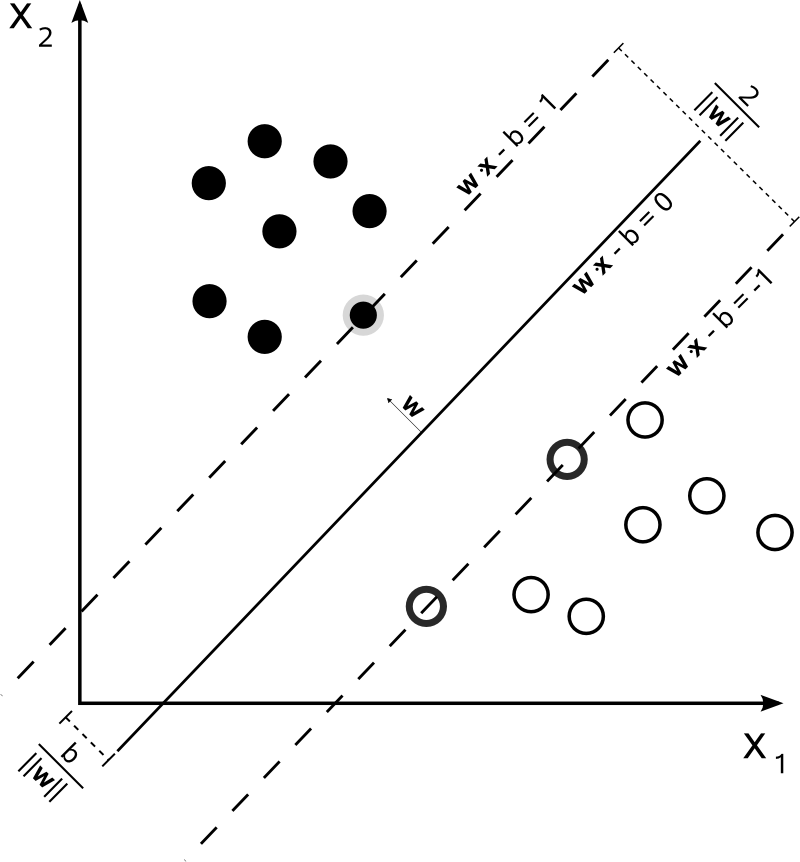
\includegraphics[width=6cm]{svm.png}
        			\caption{A support vector machine. [Public domain]}
        			\label{fig:}
  		\end{figure}
\end{frame}

%-----------------------------------------------------------------


